%%%%%%%%%%%%%%%%%%%%%%%%%%%%%%%%%%%%%%%%%%%%%%%%%%%%%%%%%%%%%%%%%%%%%%%%
% Portada oscura: identificación institucional, título, imagen de la
% superposición de respuestas a impulsos (scripts/generar_portada.py) y
% datos de autoría.
%%%%%%%%%%%%%%%%%%%%%%%%%%%%%%%%%%%%%%%%%%%%%%%%%%%%%%%%%%%%%%%%%%%%%%%%
\begin{titlepage}
\thispagestyle{empty}
\begin{tikzpicture}[remember picture, overlay]
  \coordinate (O) at (current page.south west);
  \coordinate (C) at ($(O)+(10.5cm,0)$);

  % Logotipo y cabecera institucional
  \node[anchor=north, inner sep=0] at ($(C)+(0,27.6cm)$)
    {
\includegraphics[height=1.45cm]{logo_usal_blanco.png}};
  \draw[grismedio, line width=0.35pt] ($(O)+(3.0cm,25.6cm)$) -- ($(O)+(18.0cm,25.6cm)$);
  \node[anchor=north, align=center, inner sep=0] at ($(C)+(0,25.15cm)$)
    {{\color{gris}\scshape\small\textls[140]{\Facultad\ \ ·\ \ \Titulacion}}};

  % Asignatura, tema y título
  \node[anchor=north, align=center, inner sep=0, text width=16cm] at ($(C)+(0,23.3cm)$)
    {{\color{cian}\scshape\large\textls[180]{\Asignatura}}\\[6pt]
     {\color{gris}\scshape\normalsize\textls[140]{\NumTema}}\\[20pt]
     {\color{blanco}\fontsize{30}{37}\selectfont\bfseries\TituloTema}\\[14pt]
     {\color{cian}\rule{3.2cm}{0.7pt}}\\[12pt]
     {\color{texto}\itshape\large\SubtituloTema}};

  % Respuestas a impulsos (en cascada) y su superposición
  \node[anchor=center, inner sep=0] at ($(C)+(0,10.6cm)$)
    {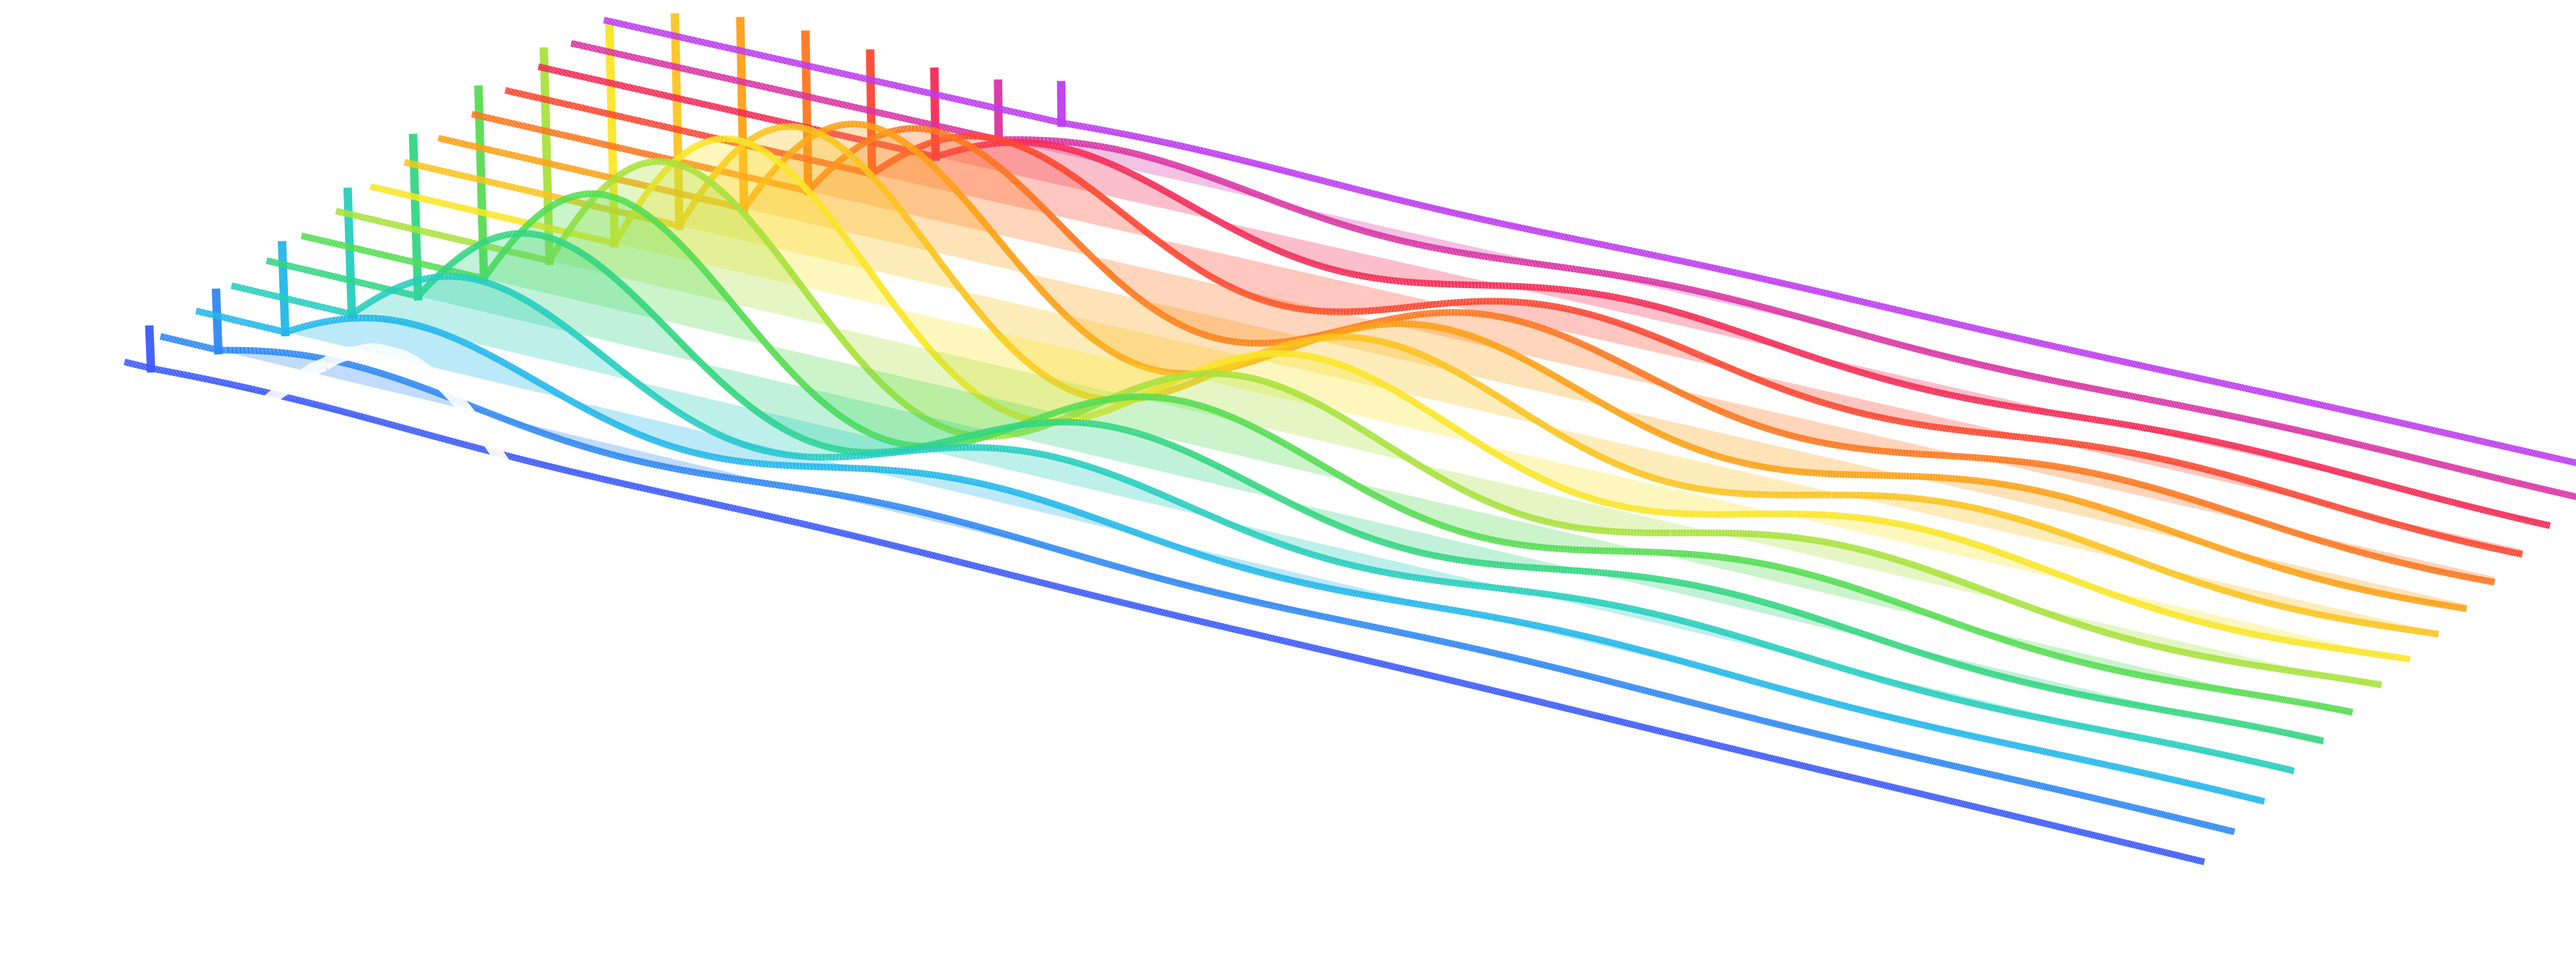
\includegraphics[width=16.4cm]{figuras/portada_superficie.png}};

  % Epígrafe: la función de Green y la solución como superposición
  \node[anchor=north, align=center, inner sep=0] at ($(C)+(0,6.4cm)$)
    {\color{texto}$\displaystyle
      \Lop_x\,G(x,\tilde x)=\delta(x-\tilde x),\qquad
      y_p(x)=\int G(x,\tilde x)\,b(\tilde x)\,\dif\tilde x$};

  % Autoría, profesorado, lugar y curso
  \draw[grismedio, line width=0.35pt] ($(O)+(3.0cm,4.2cm)$) -- ($(O)+(18.0cm,4.2cm)$);
  \node[anchor=north west, inner sep=0, align=left] at ($(O)+(3.0cm,3.75cm)$)
    {{\scshape\small\color{cian}\textls[100]{Autor}}\\[3pt]
     {\large\color{blanco}\miNombre}};
  \node[anchor=north, inner sep=0, align=center] at ($(C)+(0,3.75cm)$)
    {{\scshape\small\color{cian}\textls[100]{Profesorado}}\\[3pt]
     {\small\color{texto}\miProfesorado}};
  \node[anchor=north east, inner sep=0, align=right] at ($(O)+(18.0cm,3.75cm)$)
    {{\scshape\small\color{cian}\textls[100]{\tipotrabajo}}\\[3pt]
     {\color{gris}\miUbicacion}};
\end{tikzpicture}
\end{titlepage}
